
% This LaTeX was auto-generated from MATLAB code.
% To make changes, update the MATLAB code and republish this document.

\documentclass{article}
\usepackage{graphicx}
\usepackage{color}

\sloppy
\definecolor{lightgray}{gray}{0.5}
\setlength{\parindent}{0pt}

\begin{document}

    
    
\subsection*{Contents}

\begin{itemize}
\setlength{\itemsep}{-1ex}
   \item Question 3.3.3 Policy Evaluation
   \item Inequality Figures
\end{itemize}
\begin{verbatim}
clear
\end{verbatim}


\subsection*{Question 3.3.3 Policy Evaluation}

\begin{par}
What happens to macroeconomic aggregates (Y; K; C), to equilibrium prices (w; r) and the equilibrium distributions for earnings (1 -��)wyl, income (1 - ��)wyl + ra, assets a and consumption c.
\end{par} \vspace{1em}
\begin{verbatim}
% For the distributions, you may want to calculate Gini coefficients
% or if possible, plot the Lorenz curves, under the two different specifications.

% Is UBI welfare-improving? To answer this question you may want to compare the
% value functions v(a; y) under the two policies for some combinations of (a; y);
% or aggregate (utilitarian) social welfare

load('withoutUBI.mat')

vWage = zeros(1,2);
vRate = zeros(1,2);
vAggY = zeros(1,2);
vAggK = zeros(1,2);
vAggConsumption = zeros(1,2);
vAggValue = zeros(1,2);

vDistribution = zeros(nGridShocks*nAssets,2);
vIndEarnings = zeros(nGridShocks*nAssets,2);
vIndIncome = zeros(nGridShocks*nAssets,2);
vIndAsset = zeros(nGridShocks*nAssets,2);
vIndConsumption = zeros(nGridShocks*nAssets,2);
vIndValue = zeros(nGridShocks*nAssets,2);

vGiniCoefficientsEarnings = zeros(1,2);
vGiniCoefficientsIncome = zeros(1,2);
vGiniCoefficientsAssets = zeros(1,2);
vGiniCoefficientsConsumption = zeros(1,2);
vGiniCoefficientsValue = zeros(1,2);

%========================================

vDistribution(:,1) = vStationaryDistribution;

vWage(1) = wage;
vRate(1) = r;
vAggK(1) = capitalSupply;
vAggY(1) = capitalSupply^aalphaK * laborSupplyEffective^(1-aalphaK);

vConsumption = mConsumptionPolicy(:);
vAggConsumption(1) = vStationaryDistribution' * vConsumption;

vValue = mValue(:);
vAggValue(1) = vStationaryDistribution' * vValue;


mIndEarnings = mLaborPolicy.*vIncomeShocks';
mIndIncome = mIndEarnings + r * vGridAsset;
mIndAsset = repmat(vGridAsset,1,nGridShocks);
vIndEarnings(:,1) = mIndEarnings(:);
vIndIncome(:,1) = mIndIncome(:);
vIndAsset(:,1) = mIndAsset(:);
vIndConsumption(:,1) = vConsumption;
vIndValue(:,1)=mValue(:);
% vGiniCoefficients(1) = % to be calculated

%==========================================
load('withUBI.mat')
vDistribution(:,2) = vStationaryDistribution;

vWage(2) = wage;
vRate(2) = r;
vAggK(2) = capitalSupply;
vAggY(2) = capitalSupply^aalphaK * laborSupplyEffective^(1-aalphaK);

vConsumption = mConsumptionPolicy(:);
vAggConsumption(2) = vStationaryDistribution' * vConsumption;

vValue = mValue(:);
vAggValue(2) = vStationaryDistribution' * vValue;

mIndEarnings = (1-ttao) * mLaborPolicy.*vIncomeShocks';
mIndIncome = mIndEarnings + r * vGridAsset;
mIndAsset = repmat(vGridAsset,1,nGridShocks);

vIndEarnings(:,2) = mIndEarnings(:);
vIndIncome(:,2) = mIndIncome(:);
vIndAsset(:,2) = mIndAsset(:);
vIndConsumption(:,2) = vConsumption;
vIndValue(:,2)=mValue(:);

% vGiniCoefficients(2) = % to be calculated
\end{verbatim}


\subsection*{Inequality Figures}

\begin{verbatim}
figure
subplot(1,2,1)
vGiniCoefficientsEarnings(1) = giniFunction(vDistribution(:,1),vIndEarnings(:,1),true); % Copyright (c) 2010, Yvan Lengwiler
xlabel('share of earnings without UBI');
subplot(1,2,2)
vGiniCoefficientsEarnings(2) = giniFunction(vDistribution(:,2),vIndEarnings(:,2),true); % Copyright (c) 2010, Yvan Lengwiler
xlabel('share of earnings with UBI');
savefig('giniEarnings')


figure
subplot(1,2,1)
vGiniCoefficientsIncome(1) = giniFunction(vDistribution(:,1),vIndIncome(:,1) ,true); % Copyright (c) 2010, Yvan Lengwiler
xlabel('share of income without UBI');
subplot(1,2,2)
vGiniCoefficientsIncome(2) = giniFunction(vDistribution(:,2),vIndIncome(:,2) ,true); % Copyright (c) 2010, Yvan Lengwiler
xlabel('share of income with UBI');
savefig('giniIncome')

figure
subplot(1,2,1)
vGiniCoefficientsAssets(1) = giniFunction(vDistribution(:,1),vIndAsset(:,1),true) ;% Copyright (c) 2010, Yvan Lengwiler
xlabel('share of assets without UBI');
subplot(1,2,2)
vGiniCoefficientsAssets(2) = giniFunction(vDistribution(:,2),vIndAsset(:,2),true); % Copyright (c) 2010, Yvan Lengwiler
xlabel('share of assets with UBI');
savefig('giniAssets')

figure
subplot(1,2,1)
vGiniCoefficientsConsumption(1) = giniFunction(vDistribution(:,1),max(0,vIndConsumption(:,1)) ,true) ;% Copyright (c) 2010, Yvan Lengwiler
xlabel('share of consumption without UBI');
subplot(1,2,2)
vGiniCoefficientsConsumption(2) = giniFunction(vDistribution(:,2),max(vIndConsumption(:,2) ,0),true) ;% Copyright (c) 2010, Yvan Lengwiler
xlabel('share of consumption with UBI');
savefig('giniConsumption')

figure
subplot(1,2,1)
vGiniCoefficientsValue(1) = giniFunction(vDistribution(:,1),exp(vIndValue(:,1)),true) ;% Copyright (c) 2010, Yvan Lengwiler
xlabel('share of value exponent without UBI');
subplot(1,2,2)
vGiniCoefficientsValue(2) = giniFunction(vDistribution(:,2),exp(vIndValue(:,2)),true); % Copyright (c) 2010, Yvan Lengwiler
xlabel('share of value exponent with UBI');
savefig('giniExpValue')

table(vWage,vRate)
table(vAggY,vAggK,vAggConsumption,vAggValue)
table(vGiniCoefficientsEarnings,vGiniCoefficientsIncome,vGiniCoefficientsAssets,vGiniCoefficientsConsumption)
table(vGiniCoefficientsValue)
\end{verbatim}

        \color{lightgray} \begin{verbatim}
ans =

  1��2 table

         vWage                 vRate        
    ________________    ____________________

    1.1927    1.2169    0.039032    0.034855


ans =

  1��4 table

         vAggY               vAggK           vAggConsumption         vAggValue     
    ________________    ________________    _________________    __________________

    1.6947    1.3661    5.1197    4.2819    1.1936    0.92718    -16.159    -16.577


ans =

  1��4 table

    vGiniCoefficientsEarnings    vGiniCoefficientsIncome    vGiniCoefficientsAssets    vGiniCoefficientsConsumption
    _________________________    _______________________    _______________________    ____________________________

        0.3762    0.52759          0.34513    0.45676         0.41562    0.45973            0.2532    0.32265      


ans =

  table

    vGiniCoefficientsValue
    ______________________

      0.99003    0.97497  

\end{verbatim} \color{black}
    
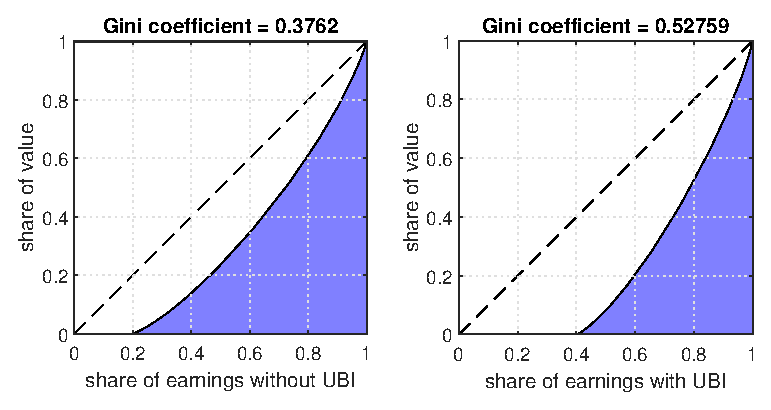
\includegraphics [width=4in]{main_7_general_eq_UBI_policy_evaluation_01.eps}

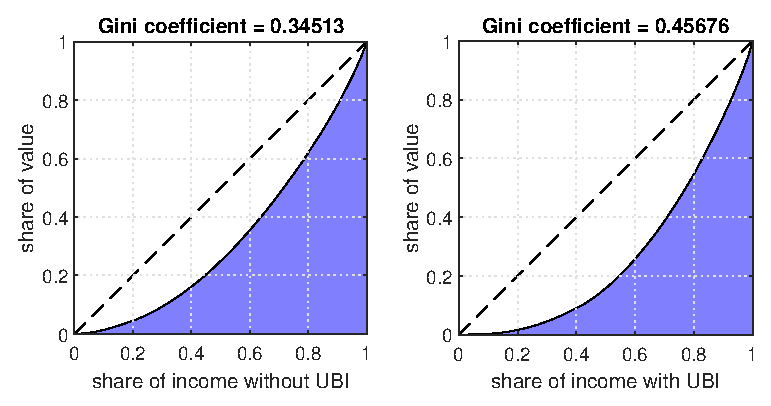
\includegraphics [width=4in]{main_7_general_eq_UBI_policy_evaluation_02.eps}

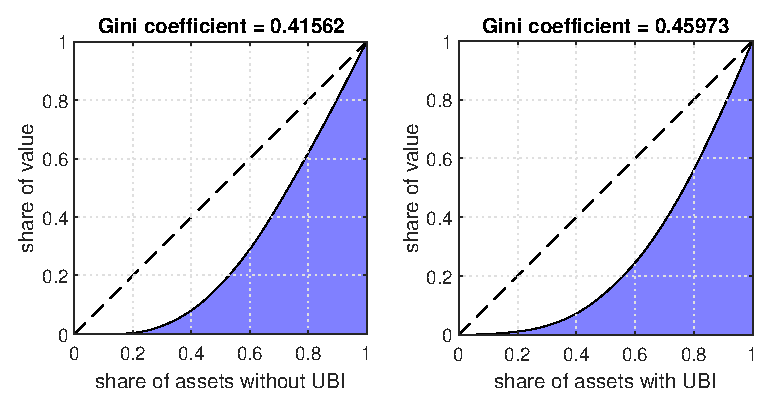
\includegraphics [width=4in]{main_7_general_eq_UBI_policy_evaluation_03.eps}

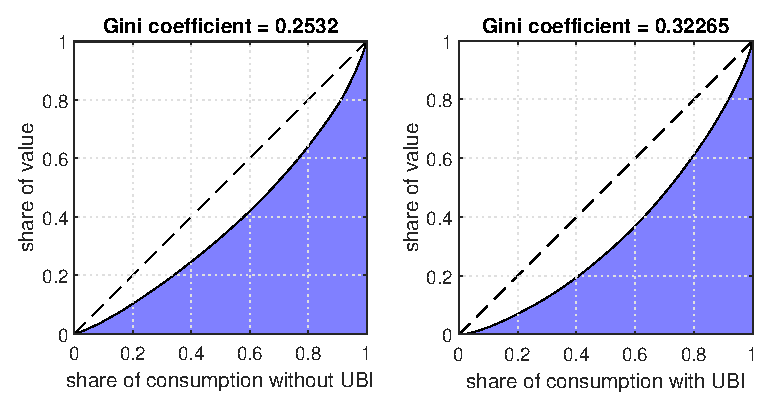
\includegraphics [width=4in]{main_7_general_eq_UBI_policy_evaluation_04.eps}

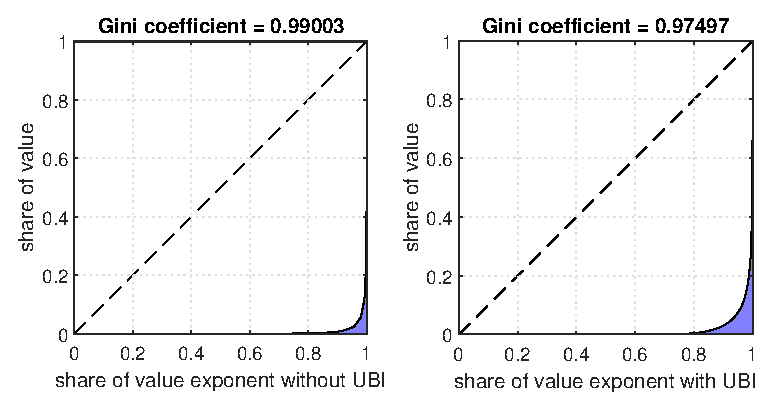
\includegraphics [width=4in]{main_7_general_eq_UBI_policy_evaluation_05.eps}



\end{document}
    
